\section{Neutrino Interaction Simulation}
\label{sec:evsim}

One of the necessary components in simulating the event rate in ND280 is the physics process model. This includes the theoretical cross sections of all neutrino scattering processes in the beam flux energy range, the propagation of produced particles through the nuclear medium and the macroscopic propagation of exiting particles through the detector. The work summarized in this Section was completed by the neutrino interaction working group of the T2K experiment.

The task of propagating particles through the detector materials is accomplished with GEANT4, a simulation software common in High Energy Physics experiments. The detector geometry is encoded into GEANT4 and the simulation software handles effects of energy loss, hadronic interactions and the magnetic field. Deposited energy in an active region of the detector is handled by proprietary software (elecSim) designed to mimic expected electronic responses of each detector. 

Before GEANT4 and the ND280 software propagate particles, the particle four vectors must be generated. A neutrino interaction simulator called NEUT\cite{neut} is responsible for determining the particles that come out of an interaction vertex. NEUT also corrects for effects of the nuclear medium. The cross section models used by NEUT and the variables that govern the interaction process amplitudes are of great interest as they affect the background and efficiency predictions required in the CC inclusive cross section measurement. A description of the parameters and the external data driven process used to assign systematic uncertainties is provided in Ref\cite{xsectn} and resummarized here.

The primary source of external data used to constrain the cross section model parameters and the corresponding uncertainties is the MiniBooNE experiment. MiniBooNE is a short-baseline neutrino experiment with several published differential cross section results including CCQE, CC1$\pi^+$, CC1$\pi^0$ and NC1$\pi^0$. The neutrino flux shape at MiniBooNE is wider than that of T2K, allowing excellent coverage of neutrino energy phase space. The MiniBooNE Cherenkov detector has a 4-$\pi$ solid angle acceptance and so covers the muon angle phase space also. Finally, the target at MiniBooNE is $CH_2$ which is similar to the carbon and oxygen targets in the P0D. Data from this experiment allows data driven constraints to be placed on model parameters governing neutrino cross sections. Some data from K2K, NOMAD and Sci-BooNE were used to cross check results and motivate conservative error assignments. Various other electron and pion scattering experiments were also used by NEUT to constrain nominal parameter values.

\subsection{Low Energy Quasi-Elastic Scattering}

The quasi-elastic scattering cross section is modeled using the Lewellyn Smith\cite{LSCCQE} formalism described in Section \ref{sec:ccqexsec}. To account for the effects of bound nucleons, the nuclei are modeled as a relativistic Fermi gas (RFG) and the density of states is defined by the Smith and Moniz\cite{RFG} model. The cross section parameters of interest are the quasi-elastic axial mass $M_A^{QE}$ and the CCQE normalization while the RFG model parameters are the Fermi momentum $p_F$ and nuclear binding energy $E_b$. The nominal values for these parameters were set to the NEUT default value as suggested by data from K2K and MiniBooNE. To assign a systematic error, a chi-squared fit was performed on existing CCQE data from MiniBooNE using only two varying parameters, $M_A^{QE}$ and a CCQE normalization factor for $E_\nu < 1.5$~GeV. The uncertainty in the MiniBooNE flux is accounted for with the CCQE parametrization used in this fit. This allows the axial mass to govern the cross section shape instead of trying to fit to an overall normalization error. The nominal prediction, post-fit prediction and MiniBooNE data is shown in Figure \ref{fig:ccqefit} as a function of reconstructed $Q^2$ and $E_\nu^{QE}$.

\begin{figure}
\centering
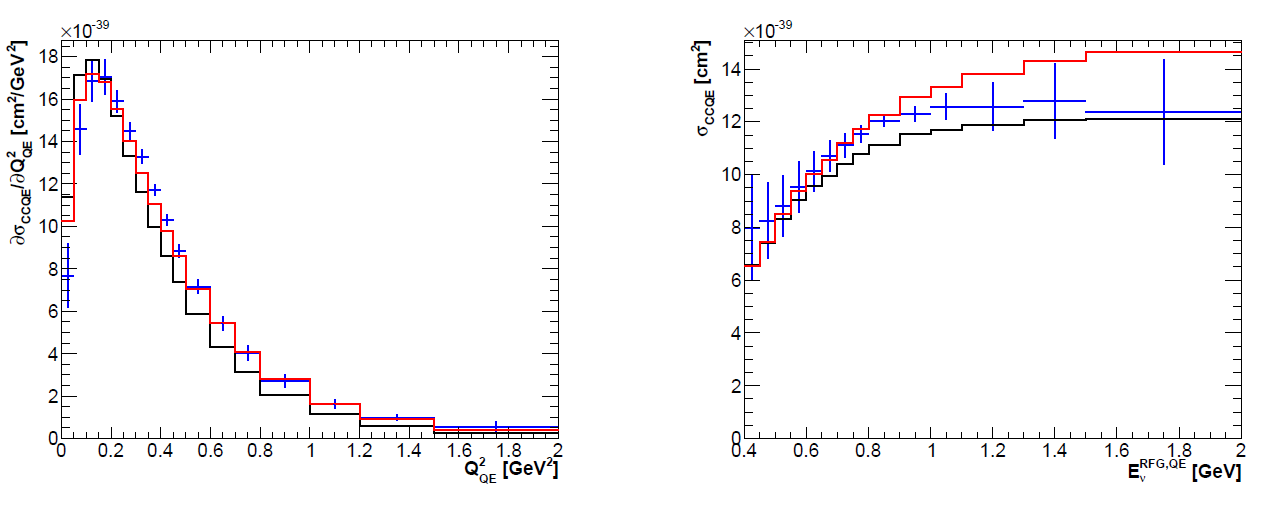
\includegraphics[width=6in]{Figures/ccqefit.PNG}
\caption{Comparison of the nominal prediction (black), post-fit prediction (red) and data (blue crosses) from the CCQE cross section measured by MiniBooNE. Left: The double differential cross section as a function of $Q^2_{QE}$. Right: The cross section as a function of the reconstructed neutrino energy.} 
\label{fig:ccqefit}
\end{figure}

Instead of using the best fit $M_A^{QE}$ value as the new central value, T2K chose to use the NEUT default as the central value and assign the the difference between nominal and fitted plus fit error ($1.64(fit) - 1.21(nom) +0.03 \approx 0.45$) value as the uncertainty\cite{xsectn}. The Fermi momentum and binding energy nominal values and errors were determined by electron scattering data in dedicated experiments. The effects of the binding energy are minimal, so the inclusive cross section measurement does not use $E_b$ to parametrize cross section error.

There is one final parameter related to the quasi-elastic scattering cross section. Instead of the RFG model, a different distribution of nucleon momentum states may be used. One such model is called the spectral function\cite{SF}. No external fits are conducted for this model. Instead, the uncertainty associated to the spectral function is a purely binary on/off switch. The difference between the CCQE cross section with the spectral function replacing the RFG model is used later to propagate the nuclear model uncertainty to the inclusive cross section measurement. Finally, the central values and errors for the quasi-elastic scattering parameters are
\begin{align}
M_A^{QE} &= 1.21\text{~GeV/}c^2  \pm 0.45\text{~GeV/}c^2 \\
\text{CCQE Norm.}(E_\nu < 1.5\text{~GeV}) &= 1.0 \pm 0.11 \\
p_F &= 217\text{~MeV/c}\pm30\text{~MeV/c}\\
\text{Spectral Function} &= \text{on/off}.
\end{align}

\subsection{Low Energy Charged-Current Resonance Production}

The resonance production cross section is modeled in NEUT using the Rein-Sehgal\cite{RS1pi} formalism described in Section \ref{sec:resxsec}. The invariant mass of the intermediate hadronic resonance $N^*$ is restricted to less than 2~GeV. To determine the angular distribution of the the pions, the RS formalism is followed for the spin 3/2 $P_{33}(1232)$ Delta resonance. All other resonances have the pion angular distribution set to isotropic in the resonance rest frame. The RS formalism is also used to calculate the $\gamma$, $K$ and $\eta$ production rates by switching out the decay amplitude portion of the cross section formula to the appropriate values while keeping the resonance production amplitude the same.

\begin{figure}
\centering
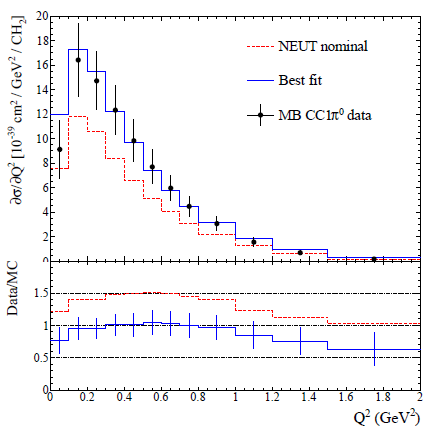
\includegraphics[width=2in]{Figures/1pifit1.PNG}
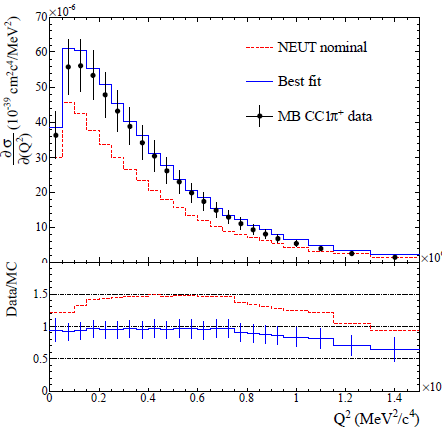
\includegraphics[width=2in]{Figures/1pifit2.PNG}
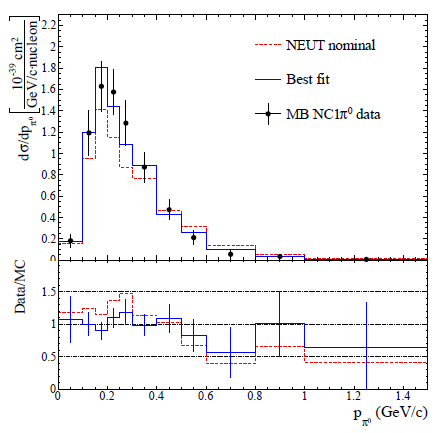
\includegraphics[width=2in]{Figures/1pifit3.PNG}
\caption{Fitted spectra of the nominal prediction (red), post-fit prediction (blue) and data (black crosses) from the differential pion production cross sections measured by MiniBooNE. Left: Differential CC1$\pi^0$ cross section as a function of $Q^2$. Middle: Differential CC1$\pi^+$ cross section as a function of $Q^2$. Right: Differential NC1$\pi^0$cross section as a function of the pion momentum. In all three plots, the bottom panel shows the data/MC ratios for the nominal MC (red) and post-fit MC (blue).} 
\label{fig:1pifit}
\end{figure}

The parameters governing single pion production rates were constrained using a joint fit to MiniBooNE data sets for charged-current $\pi^0$ (CC$\pi^0$), charged current single $\pi^+$ (CC$1\pi^+$) and neutral current $\pi^0$ production. There are nine parameters that are varied in the joint fit. The resonant axial mass $M_A^{RES}$ is described in Section \ref{sec:resxsec}. Two shape parameters, ``W shape" and ``CC other shape", modify the NC1$\pi^0$ pion momentum and reconstructed neutrino energy in various CC interactions respectively. The remaining five parameters are all normalization parameters on specific interaction channels. The nominal prediction, post-fit prediction and MiniBooNE data is shown in Figure \ref{fig:1pifit} for the three pion production data sets. Most of the normalization parameters and both of the shape parameters affect neither the background nor the signal in any appreciable way for the CC inclusive measurement and are therefore neglected in this study. The central values and assigned errors of the important parameters from the single pion external data fit are
\begin{align}
M_A^{RES} &= 1.16\text{~GeV/}c^2\pm 0.11\text{~GeV/}c^2\\
\text{CC}1\pi\text{~Norm.}(E_\nu < 2.5\text{~GeV}) &= 1.63\pm0.43
\end{align}
with the full nine parameter fit covariance shown in Figure \ref{fig:xseccorr}.

\begin{figure}
\centering
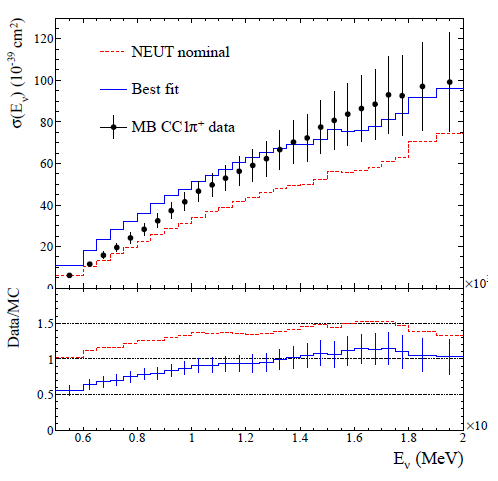
\includegraphics[width=3in]{Figures/1pienushp1.PNG}
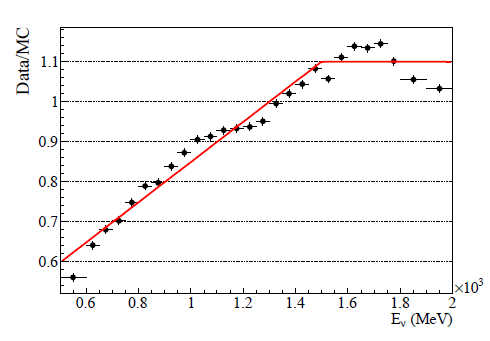
\includegraphics[width=3in]{Figures/1pienushp2.PNG}
\caption{Left: CC1$\pi^+$ cross section with the nominal prediction (red), post-fit prediction (blue) and data (black crosses) from MiniBooNE. The bottom panel is the data to MC ratios for the nominal MC (red) and post-fit MC (blue). The post-fit result overshoots the data at low energy and then undershoots it at high energy. Right: Linear reweighting function fit to the data/MC ratio for post-fit MC. This function by design corrects the data and MC disagreement.}
\label{fig:cc1pishp}
\end{figure}

\begin{figure}
\centering
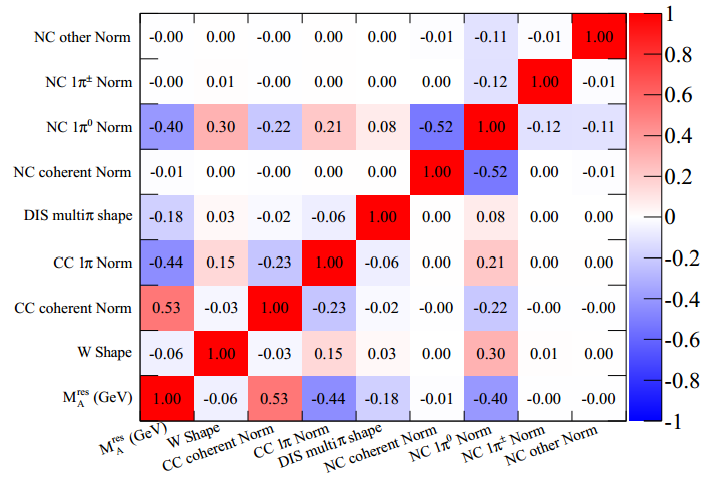
\includegraphics[width=6in]{Figures/xseccorr.png}
\caption{The correlation matrix for cross section parameters used in the single pion fits\cite{xsectn}.}
\label{fig:xseccorr}
\end{figure}

The fit results do not fully explain the MiniBooNE CC1$\pi^+$ data as a function of neutrino energy (see Figure \ref{fig:cc1pishp}). To parametrize this disagreement, a shape function is introduced that is simply a linear fit to the data to MC ratio in each neutrino energy bin. This empirical reweight function is called ``MiniBooNE CC1$\pi E_\nu$ Shape" and is show on the right plot in Figure \ref{fig:cc1pishp}. Like the spectral function, the cross section measurement uncertainty is propagated by either applying or not applying the function. We denote the ``variation" of this parameter as on or off:
\begin{equation}
\text{MiniBooNE CC1}\pi\text{~E}_\nu\text{~Shape} = on/off.
\end{equation}

\subsection{High Energy QE/1$\pi$, Pion-less Delta Decay and Other Processes}

Fits to the MiniBooNE data sets cannot constrain parameters describing cross sections at neutrino energies $>2.5$~GeV due to the limits of the MiniBooNE flux. Two CCQE normalization parameters are assigned to the high energy tail, one for neutrino energies between 1.5~GeV and 3.5~GeV (CCQE E2), and the other for energies above 3.5~GeV (CCQE E3). The observed discrepancy between the NOMAD CCQE measurement and the low energy MiniBooNE CCQE measurement is used to assign a $30\%$ error on both normalization parameters. A similar normalization parameter is also assigned to the high energy pion production cross section (CC1$\pi$ E2). Using the data to MC ratio of the MiniBooNE CC1$\pi$ cross section in the 2~GeV neutrino energy bin, CC1$\pi$ E2 is assigned an error of $40\%$.

In NEUT, $20\%$ of delta resonance production processes do not have an decay pion. This process, called pion-less delta decay (PDD), can cause misidentification of single pion events as quasi-elastic scattering. Fortunately an inclusive measurement is mostly insensitive to this effect. The PDD rate is assigned a very conservative error of $100\%$. As the nominal rate of PDD is $20\%$, this error translates to $0.2\pm0.2$.

Neutral current processes such as elastic scattering, $\gamma$ / $\eta$ / $K$ resonant production, single-pion/multi-pion production and deep-inelastic scattering are lumped into the ``NC Other" category and parametrized by a normalization factor. These interactions have almost no contribution to the CC inclusive cross section and are also very poorly constrained by the MiniBooNE NC1$\pi^0$ data. The NC Other normalization parameter is assigned a rough $30\%$ error. 

When a pion is produced from a neutrino interaction with a nucleus as a whole (instead of a singular nucleon), the process is called CC coherent pion production. In the 1~GeV energy regime, external experiments observe no CC coherent pion production at the $90\%$ confidence level. A CC coherent normalization parameter is assigned to this process with an error of $100\%$. As there is absolutely no contribution from this channel in the inclusive event selection, the NC coherent normalization parameter is neglected. 

To summarize, the normalization parameter central values and uncertainties are:
\begin{align}
\text{CCQE E2 Norm.}(1.5\text{~GeV} < E_\nu < 3.5\text{~GeV}) &= 1.0\pm0.3\\
\text{CCQE E3 Norm.}(3.5\text{~GeV} < E_\nu) &= 1\pm0.3\\
\text{CC}1\pi\text{~E2 Norm.}(E_\nu > 2.5\text{~GeV}) &= 1.0\pm0.4\\
\text{Pionless Delta Decay} &= 0.2 \pm 0.2\\
\text{NC Other Norm.} &= 1.0 \pm 0.3\\
\text{CC Coh.~}\pi\text{~Prod. Norm.} &= 1.0 \pm 1.0.
\end{align}

\subsection{Deep Inelastic Scattering}

The formalism for calculating the CC deep inelastic scattering cross section is summarized in Section \ref{sec:disxsec} by using the quark parton model. NEUT integrates the DIS differential cross section for hadronic system invariant mass (W) over 1.3~GeV. The parton distribution functions are taken from GRV98, a software routine based on Ref\cite{GRV98}. NEUT also folds the probability of finding a multi-pion process for W$<2$~GeV into the DIS cross section. The mean of the pion multiplicity is estimated using data from the Fermilab 15-foot bubble chamber experiment and is given by
\begin{equation}
\left<N_\pi\right> = 0.09+1.83 \text{ln(W$^2$)}.
\end{equation}
The kinematics of DIS events for W$>2$~GeV are simulated by the PYTHIA/Jetset software that are dedicated to generate high energy interactions. 

\begin{figure}
\centering
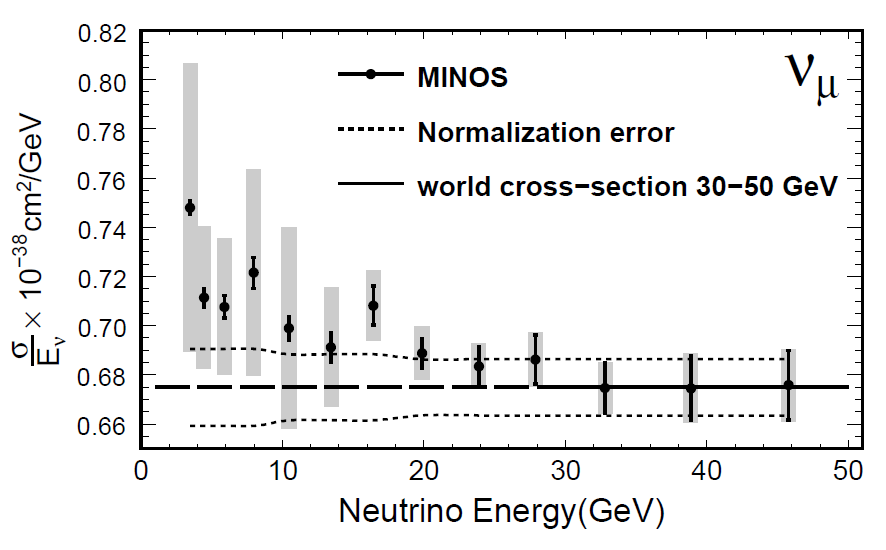
\includegraphics[width=6in]{Figures/disminos.PNG}
\caption{Total CC $\nu_\mu$ inclusive cross section measured by the MINOS experiment as a function of neutrino energy. The error from the lowest energy bin is on the order of $10\%$.} 
\label{fig:disminos}
\end{figure}

Data from a MINOS CC inclusive cross section measurement\cite{ccminos} shows that the error at 4~GeV neutrino energy is on the order of $10\%$ (see Figure \ref{fig:disminos}). The uncertainty on the DIS and multi-pion production processes is parametrized by a normalization factor and modeled in an energy dependent manner: $\delta_{DIS} = 0.4/E_\nu$. This yields a central value and error of
\begin{equation}
\text{DIS/Multi-}\pi\text{~Shape} = 1 \pm 0.4.
\end{equation}

\subsection{Final State Interactions}

Mesons and hadrons produced by neutrino-nucleon scattering can interact with the nuclear medium on their way out of the nucleus. Therefore, the observed particles are often not the original particles produced by the neutrino interaction, an effect referred to as final state interactions (FSI). NEUT simulates FSI with a cascade model that steps the primary interaction through small units of length in the nucleus. At each step, the simulation checks to see whether an FSI occurred.

Pion, kaon/eta and hadron interactions are all treated a little differently by NEUT. For pions, the FSI that are considered are inelastic scattering, charge exchange and absorption. In the case of high energy pions, particle production is also considered. Interaction probabilities of pions with energies below 500~MeV are calculated in NEUT while interaction probabilities of pions with higher momentum are taken from pion-nucleon scattering experiments. Kaon interaction rates are extracted from kaon scattering experiments and $\eta$ absorption rates are calculated by NEUT. The only change for nucleon rescattering is that the considered FSI are elastic scattering or single/double delta production. The rates are extracted from nucleon-nucleon scattering experiments. Of the processes affected by FSI, CC resonant pion production has the highest contribution to the inclusive cross section.

\begin{figure}
\centering
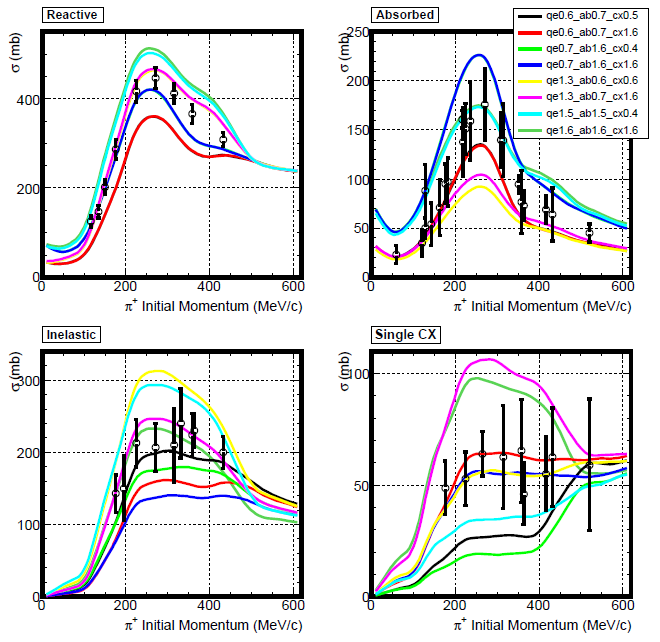
\includegraphics[width=6in]{Figures/fsifit.PNG}
\caption{MC predictions from eight variations of the set of three low energy FSI parameters. The curves are overlayed with pion scattering data (inelastic data refers to quasi-elastic scattering). The legend corresponds to the parameters in the text as follows: qe is FSIQE, ab is FSIABS and cx is FSICX. } 
\label{fig:fsifit}
\end{figure}

Two sets of scaling parameters govern the pion-nucleon interaction probabilities in NEUT, one set for the low energy pions and another for high energy pions. One parameter in each set corresponds to one of three interaction modes: quasi-elastic scattering, single charge exchange and pion absorption. In the case of the pion absorption, the high energy and low energy sets use the same scale parameter. The high energy set also includes a parameter for pion production. This yields a total of six parameters to characterize pion FSI. The three low energy FSI parameters for absorption (FSIABS), QE scattering (FSIQE) and charge exchange (FSICX) were varied simultaneously and the pion scattering predictions were resimulated. The predictions from each three-parameter variation were compared with the low energy pion scattering data and eight combinations of values were selected to approximately cover the 1-sigma error in the available external data. The results of the low energy parameter set variations are shown in Figure \ref{fig:fsifit}. To span the errors in the high energy data, only two combinations of the three high energy parameters were necessary. The high energy parameters are QE scattering (FSIQEH), charge exchange (FSICXH) and pion production (FSIINEL). The total number of FSI parameter value combinations is therefore 16. The 16 variations are used later to propagate FSI systematic uncertainties to the inclusive cross section measurement. Fortunately, as an inclusive measurement mostly ignores what happens to the pion, the effects are small.
